\documentclass{article}

\usepackage{amssymb,amsmath,amsfonts,amstext}
\usepackage{graphicx}
%\usepackage{subfigure}
\usepackage{mathtools}
\usepackage{stmaryrd}
\usepackage{color}
\usepackage{verbatim}
\usepackage{amsthm}
\usepackage{esint}
\usepackage{caption,subcaption}
\usepackage{titlesec}
\setcounter{secnumdepth}{4}
\usepackage{geometry}
\geometry{left=3.18cm,right=3.18cm,top=2.54cm,bottom=2.54cm}


\title{Neural network}
\author{Xiaoguai Li}
\date{}

\begin{document}


\maketitle

\section{Goal}
Generate a set of N observations using a Latin Hypercube Sampling of $f(x, y) = cos(\pi x) cos(\pi y), x, y \in [50, 54]$ and train a deep neural network with two hidden layers, 50 neurons per layer, and a hyperbolic tangent activation function to approximate $f(x,y)$. Plot the approximation error in the L2 norm as the number of training points is increased.

\section{Results}
The following figures in Fig.1 are directly generated by functionApproximatioin\_NN, which is the main script. It imports NeuralNetwork from models numpy.py. At the beginning of functionApproximatioin\_NN.py, number of training data can be defined.
1000 test data is used. 40000 iteration is used to train the model. Batch size is full. Fig.2
shows the error of prediction with respect to different numbers of training data. This plot shows
convergence, which is not guaranteed theoretically.
\begin{figure}[htbp]
\center
    \begin{subfigure}{0.45\textwidth}
        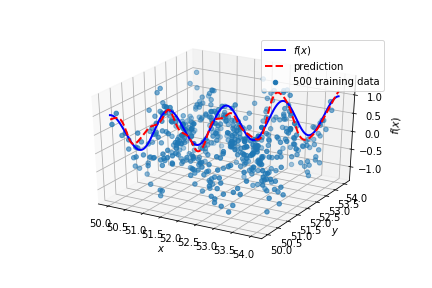
\includegraphics[width=\textwidth]{figures/500TrainingData}
        \caption{500 Training Data}
    \end{subfigure}
    ~ %add desired spacing between images, e. g. ~, \quad, \qquad, \hfill etc. 
      %(or a blank line to force the subfigure onto a new line)
    \begin{subfigure}{0.45\textwidth}
        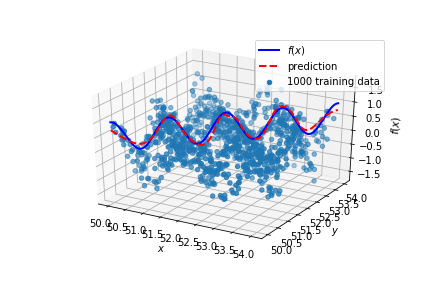
\includegraphics[width=\textwidth]{figures/1000TrainingData}
        \caption{1000 Training Data}
    \end{subfigure}
        ~ %add desired spacing between images, e. g. ~, \quad, \qquad, \hfill etc. 
      %(or a blank line to force the subfigure onto a new line)
    \begin{subfigure}{0.45\textwidth}
        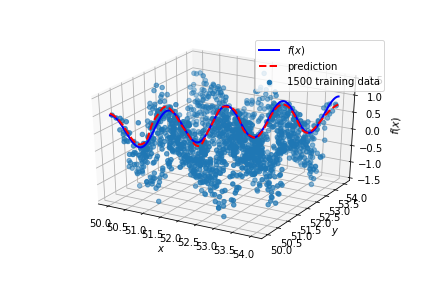
\includegraphics[width=\textwidth]{figures/1500TrainingData}
        \caption{1500 Training Data}
    \end{subfigure}
~ %add desired spacing between images, e. g. ~, \quad, \qquad, \hfill etc. 
      %(or a blank line to force the subfigure onto a new line)
    \begin{subfigure}{0.45\textwidth}
        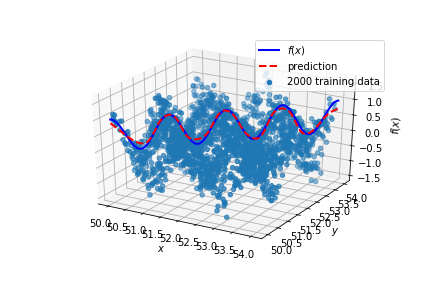
\includegraphics[width=\textwidth]{figures/2000TrainingData}
        \caption{2000 Training Data}
    \end{subfigure}
\end{figure}

     \addtocounter{figure}{-1}  
\begin{figure}[htbp]
\center

    \begin{subfigure}{0.45\textwidth}
        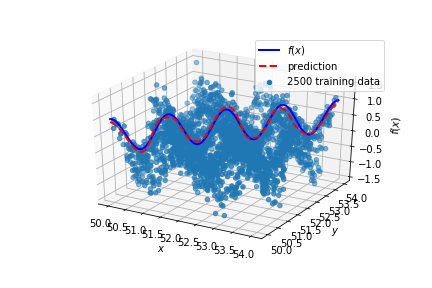
\includegraphics[width=\textwidth]{figures/2500TrainingData}
           \addtocounter{subfigure}{4}  
        \caption{2500 Training Data}
    \end{subfigure}
        ~ %add desired spacing between images, e. g. ~, \quad, \qquad, \hfill etc. 
      %(or a blank line to force the subfigure onto a new line)
    \begin{subfigure}{0.45\textwidth}
        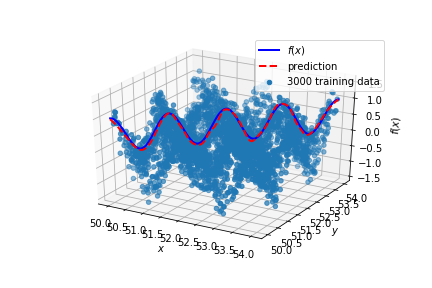
\includegraphics[width=\textwidth]{figures/3000TrainingData}
        \caption{3000 Training Data}
    \end{subfigure}
~ %add desired spacing between images, e. g. ~, \quad, \qquad, \hfill etc. 
      %(or a blank line to force the subfigure onto a new line)
    \begin{subfigure}{0.45\textwidth}
        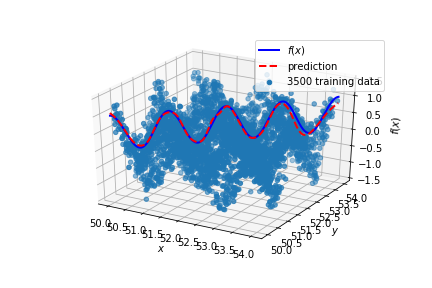
\includegraphics[width=\textwidth]{figures/3500TrainingData}
        \caption{3500 Training Data}
    \end{subfigure}
        ~ %add desired spacing between images, e. g. ~, \quad, \qquad, \hfill etc. 
      %(or a blank line to force the subfigure onto a new line)
    \begin{subfigure}{0.45\textwidth}
        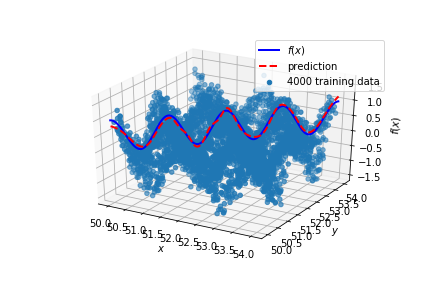
\includegraphics[width=\textwidth]{figures/4000TrainingData}
        \caption{4000 Training Data}
    \end{subfigure}
~ %add desired spacing between images, e. g. ~, \quad, \qquad, \hfill etc. 
      %(or a blank line to force the subfigure onto a new line)
    \begin{subfigure}{0.45\textwidth}
        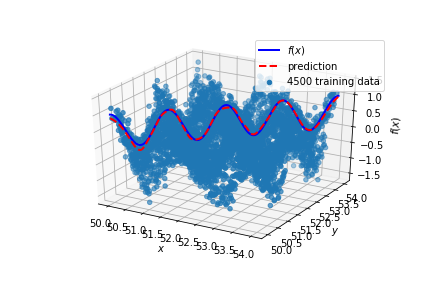
\includegraphics[width=\textwidth]{figures/4500TrainingData}
        \caption{4500 Training Data}
    \end{subfigure}
        ~ %add desired spacing between images, e. g. ~, \quad, \qquad, \hfill etc. 
      %(or a blank line to force the subfigure onto a new line)
    \begin{subfigure}{0.45\textwidth}
        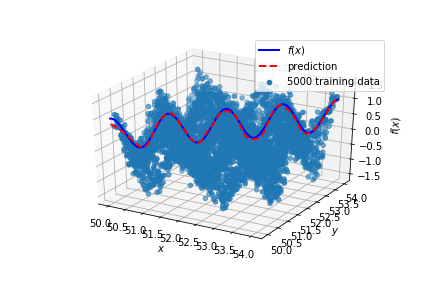
\includegraphics[width=\textwidth]{figures/5000TrainingData}
        \caption{5000 Training Data}
    \end{subfigure}
    \caption{Prediction results with different numbers of training data}

\end{figure}
%%%%%%%%%%

%\section{Part II}
%The following figures in Fig.3 are directly plotted from my codes. The main script is Assignment3\_2.py. It imports NeuralNetwork from PDEsolver\_tf.py.  At the beginning of Assignment3\_2.py, number of training data can be defined.

%1000 test data is used. 40000 iteration is used to train the model. Batch size is full. Fig.4 shows the error of prediction with respect to different numbers of training points. This plot shows convergence again.


\begin{figure}
    \center
    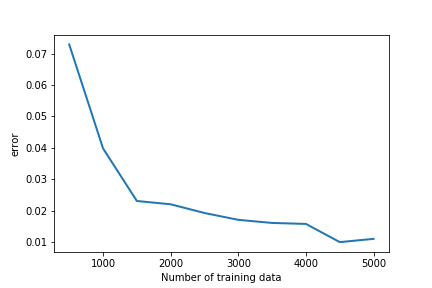
\includegraphics[width=0.6\textwidth]{figures/error.png}
    \caption{Prediction error decreases with increasing number of training data}
\end{figure}


\end{document}



